\section{Web hacking}

\subsection{Unicorn 1 (Unfinished) (100p)}
\addtocounter{unfinished}{100}
\url{http://julie.hackingarena.no:801}

\textbf{Solution:}\\
Beginning this task was quite difficult. 
But I eventually managed to find the \texttt{robots.txt} file and the \texttt{2020} directory.

\begin{center}
    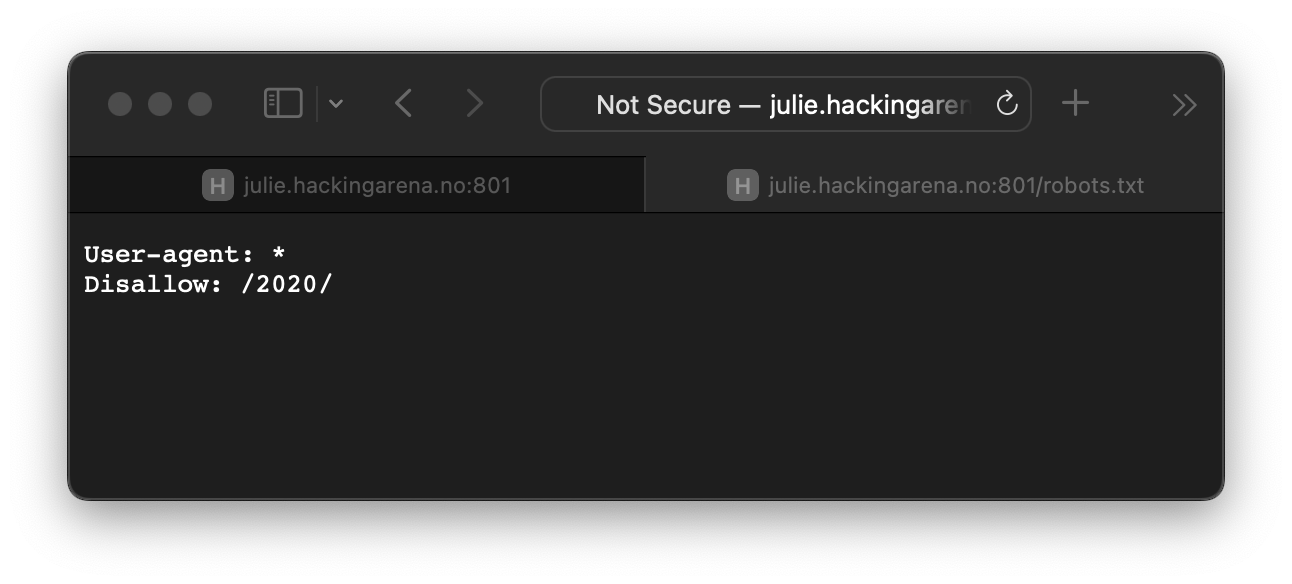
\includegraphics[width=15cm]{img/Web hacking/Unicorn 1/Screenshot 2023-11-24 at 22.15.51.png}
\end{center}

In the \texttt{2020} directory I found a file called \texttt{index.inc}. 

\begin{center}
    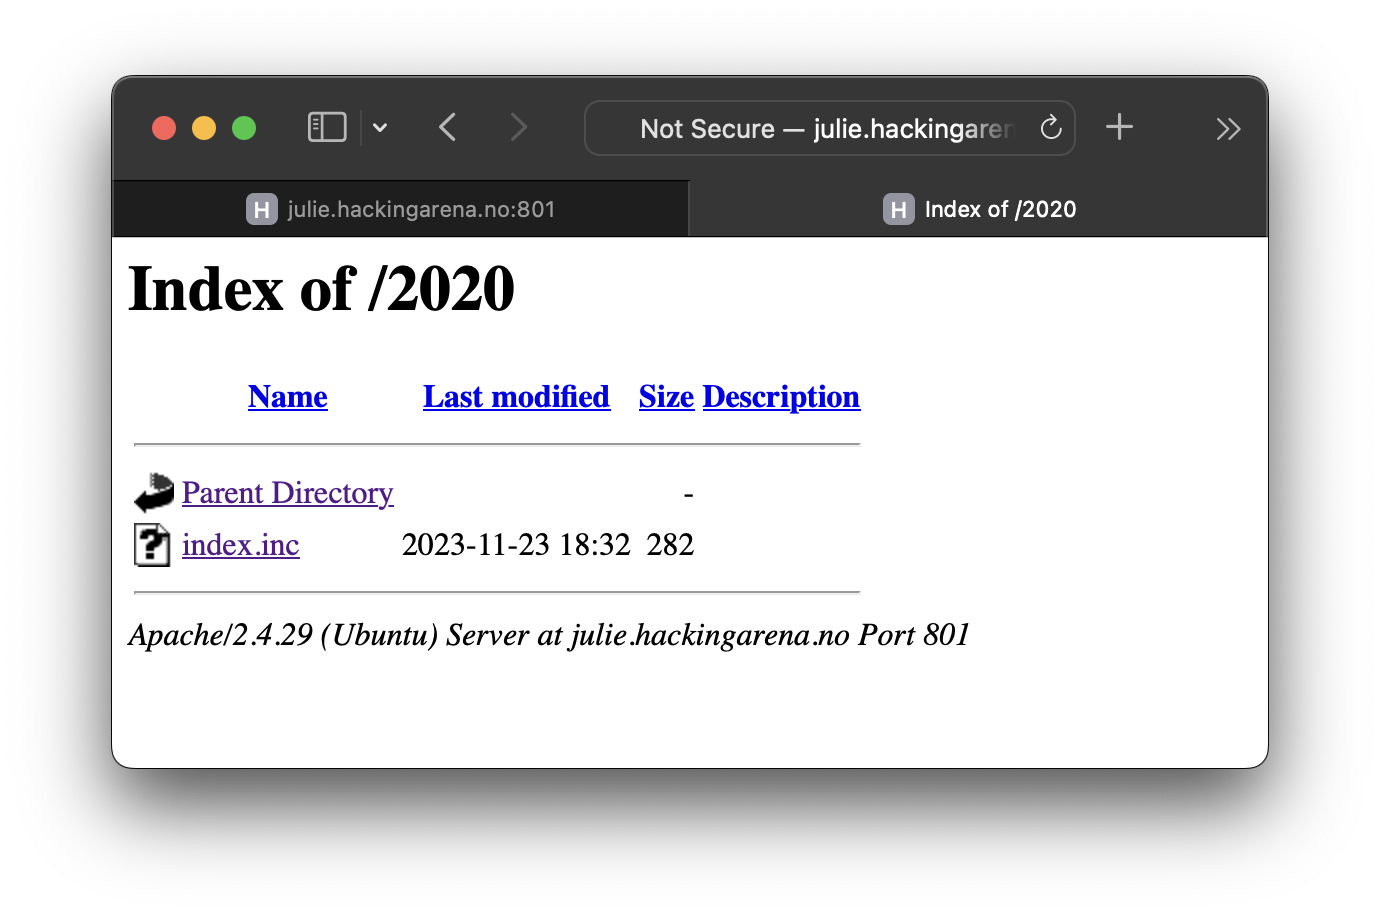
\includegraphics[width=14cm]{img/Web hacking/Unicorn 1/Screenshot 2023-11-24 at 22.17.38.png}
\end{center}

It contained the following code:

\begin{center}
    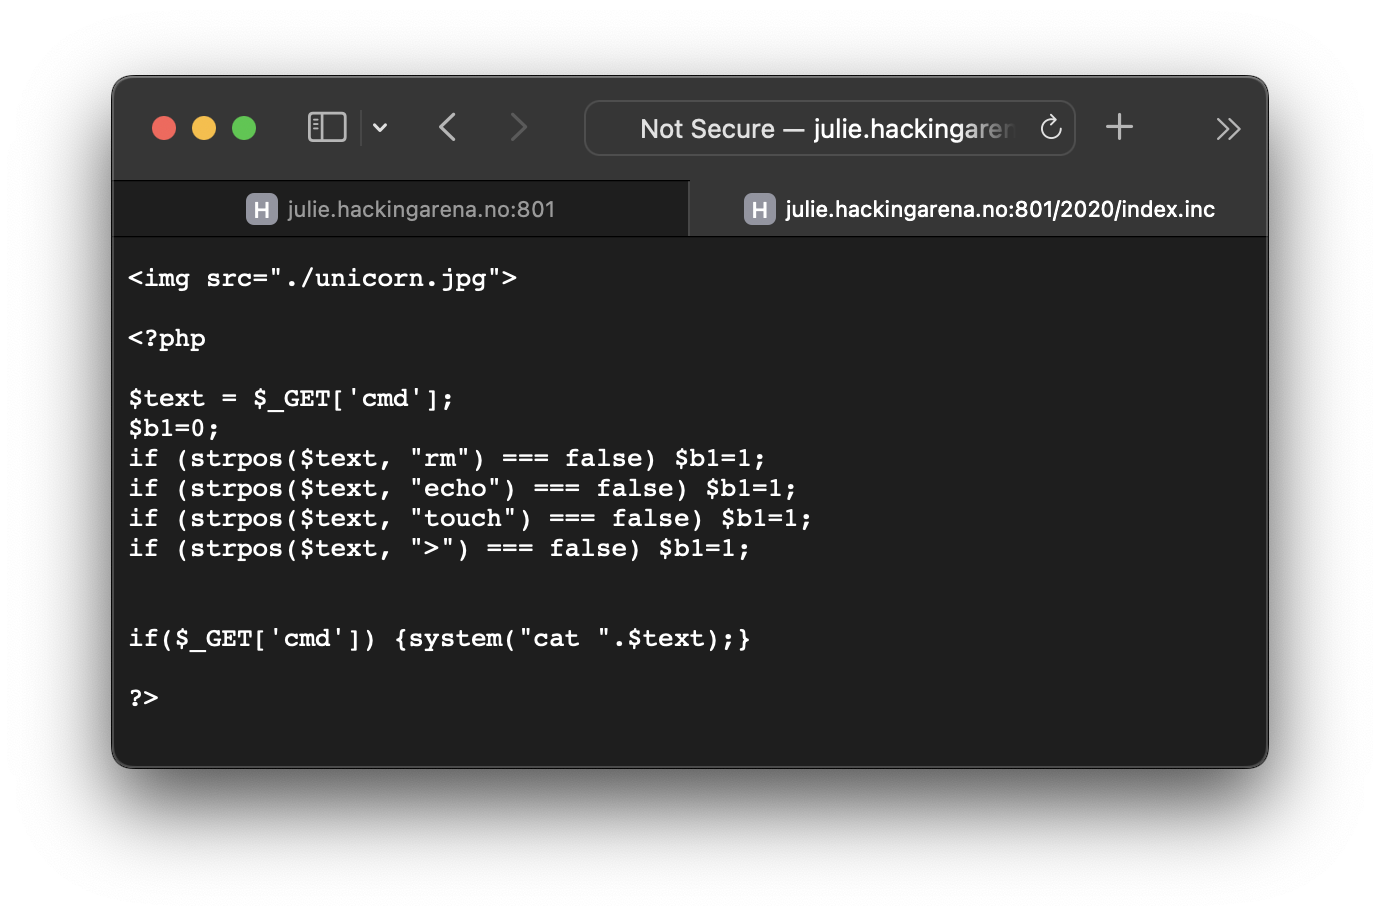
\includegraphics[width=15cm]{img/Web hacking/Unicorn 1/Screenshot 2023-11-24 at 22.17.43.png}
\end{center}

At this point I figured that the next step was to locate the flag file, but when searching known directories I couldn't find it.
I figured that since everything passed to \texttt{cmd} was being added as arguments to \texttt{cat} all that was needed was the location of the flag file.
But using commands like \texttt{ls -la} and \texttt{find / -name flag} didn't work either.

\newpage
\subsection{Tricky login (100p)}
\addtocounter{points}{100}
Well, this is a tricky login here: 
\\\url{http://julie2.hackingarena.no:803}

\textbf{Solution:}\\
When trying to login with the username \texttt{admin} and a random password I noticed that I got a output on the site. This indicated that the site might be vulnerable to an SQL injection.

\begin{center}
    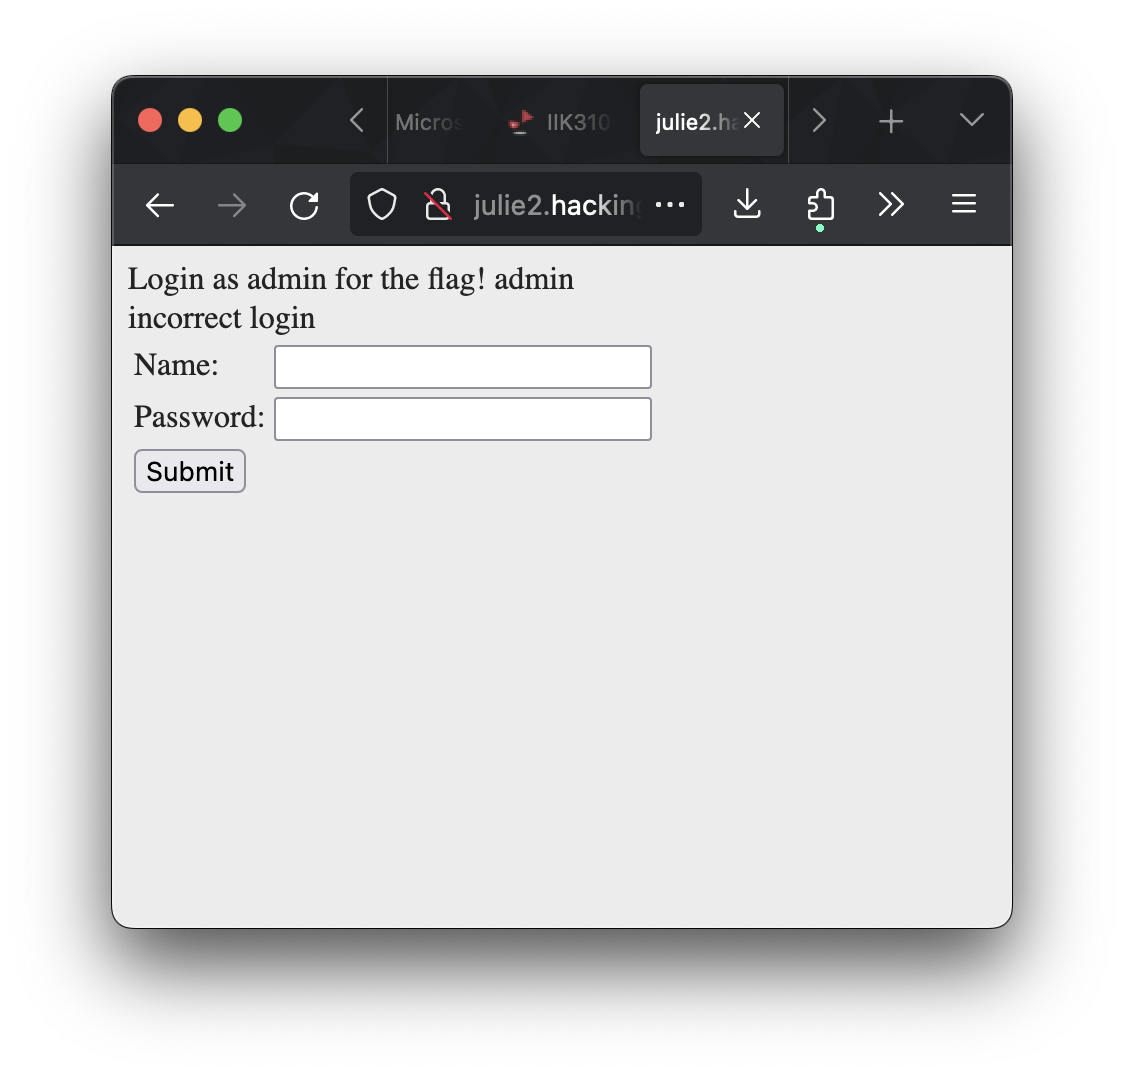
\includegraphics[width=11cm]{img/Web hacking/Tricky login/Screenshot 2023-11-24 at 16.20.45.png}
\end{center}

Using sqlmap i tried to check for vulnerabilities with the command \\\texttt{sqlmap -u "http://julie2.hackingarena.no:803" --data="username=admin\&passwd=pass"}
but that didn't result in anything. So I tried to increase the level of the test with the command 
\\\texttt{sqlmap -u "http://julie2.hackingarena.no:803" --data="username=admin\&passwd=pass" --level=2} 
and that resulted in finding a vulnerability in the username field.
I then ran the command
\\\texttt{sqlmap -u "http://julie2.hackingarena.no:803" --current-db  --data="username=admin" --tables}
to find the name of the database and the tables in it. 
This resulted in the following output:

\begin{center}
    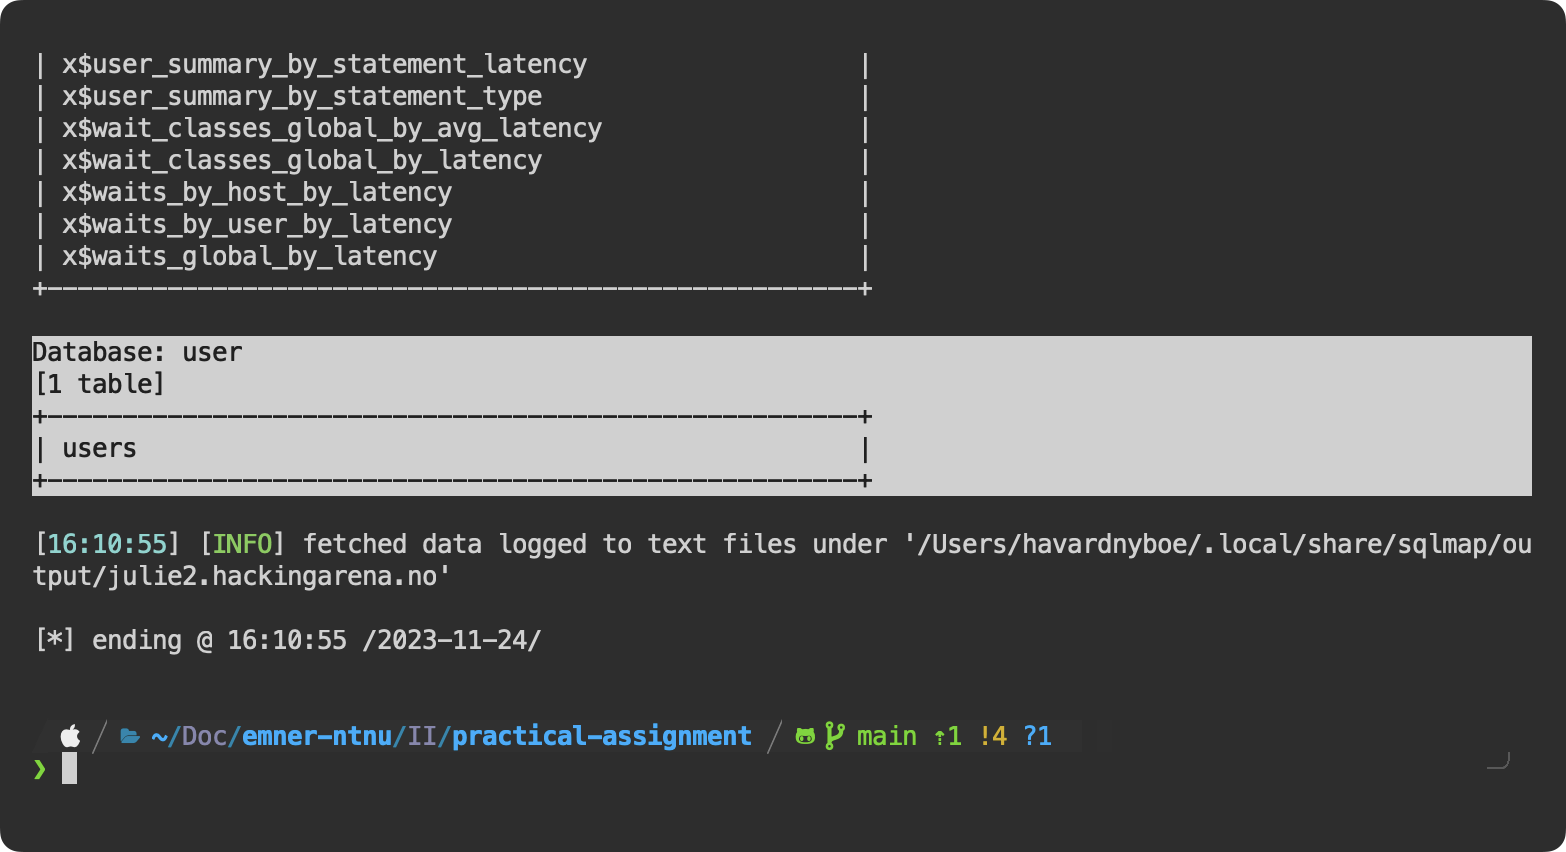
\includegraphics[width=15cm]{img/Web hacking/Tricky login/Screenshot 2023-11-24 at 16.11.07.png}
\end{center}

Assuming the users were stored in the database \texttt{user} and the table \texttt{users} I ran the command
\\\texttt{sqlmap -u "http://julie2.hackingarena.no:803" --current-db  --data="username=admin" --tables -D user -T users --dump}
to dump the users in the table \texttt{users} in the database \texttt{user}.
After that I got a prompt asking if I wanted to crack the hashes of the passwords for the users. I proceeded with that and using the default dictionary file from sqlmap I got the following output:

\begin{center}
    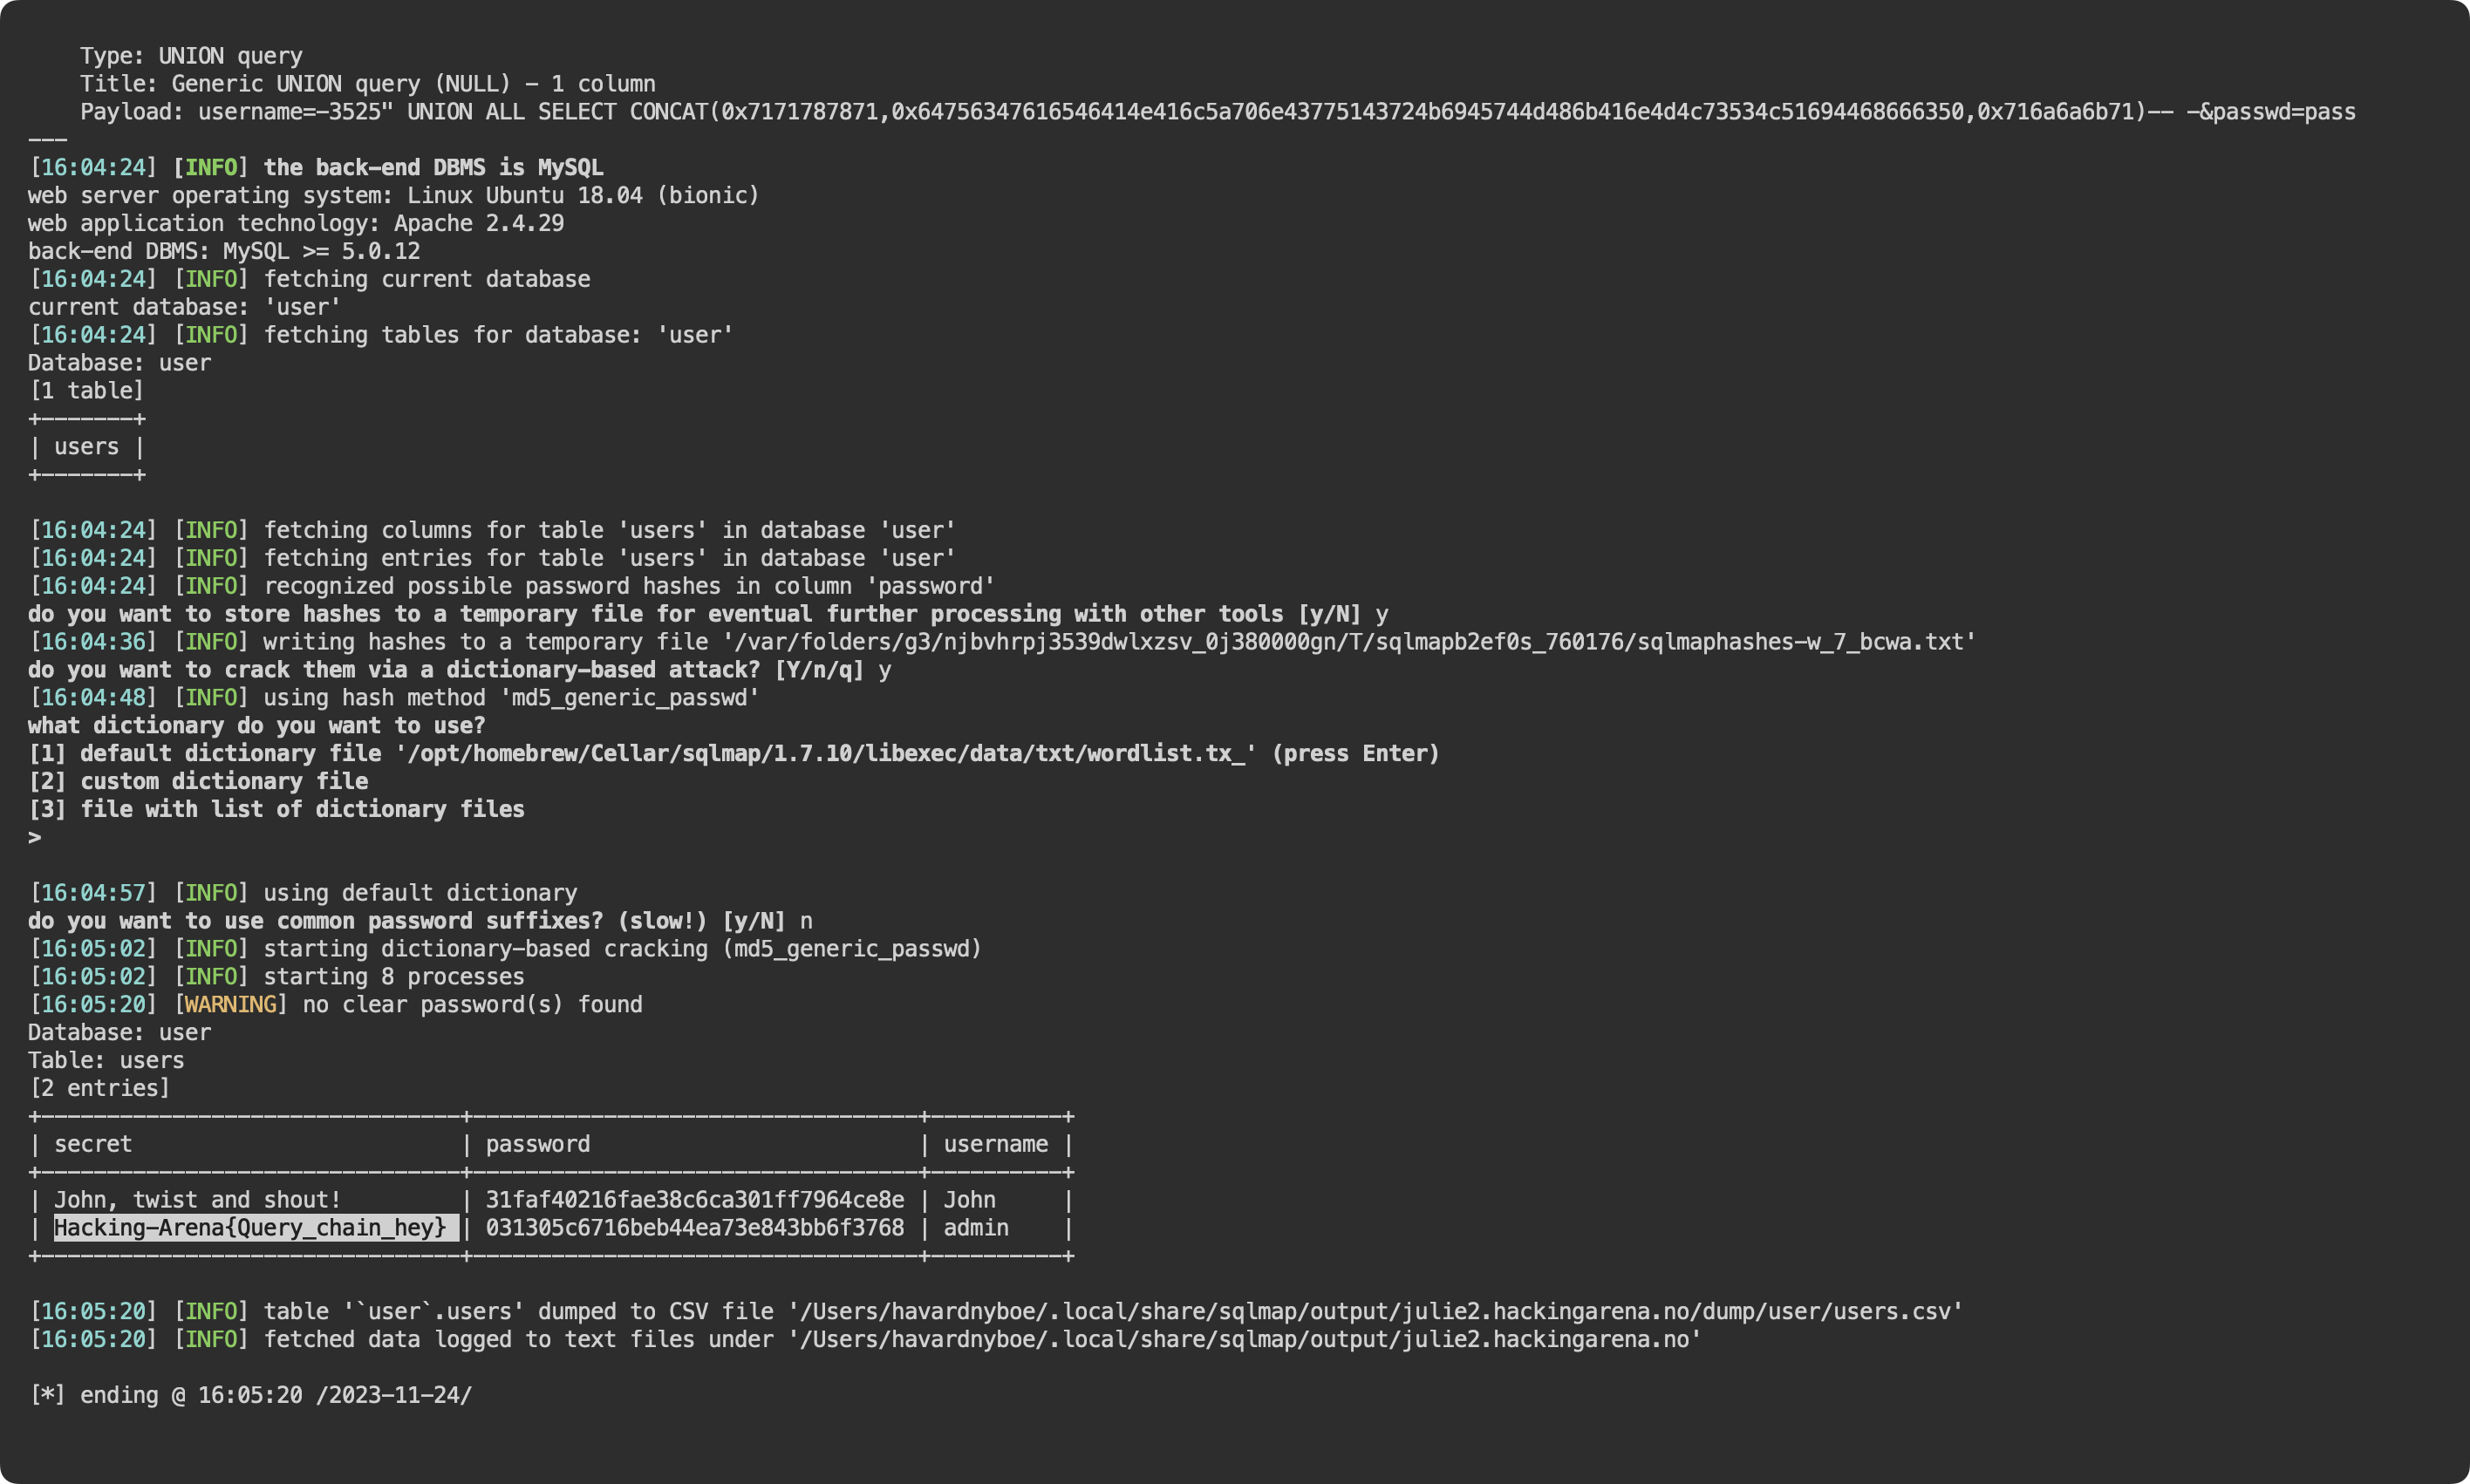
\includegraphics[width=15cm]{img/Web hacking/Tricky login/Screenshot 2023-11-24 at 16.09.41.png}
\end{center}

The flag was the password for the user \texttt{admin}, which was \texttt{Hacking-Arena\{Query\_chain\_hey\}}.

\newpage
\subsection{Order a Unicorn (100p)}
\addtocounter{points}{100}
Do you want to order a Unicorn?
\\Well, let's try it: \url{http://julie2.hackingarena.no:804}

\textbf{Solution:}\\
First I used the php filter \texttt{php://filter/convert.base64-encode/resource=index.php} to get the base64 encoded source code of the index.php file. 

\begin{center}
    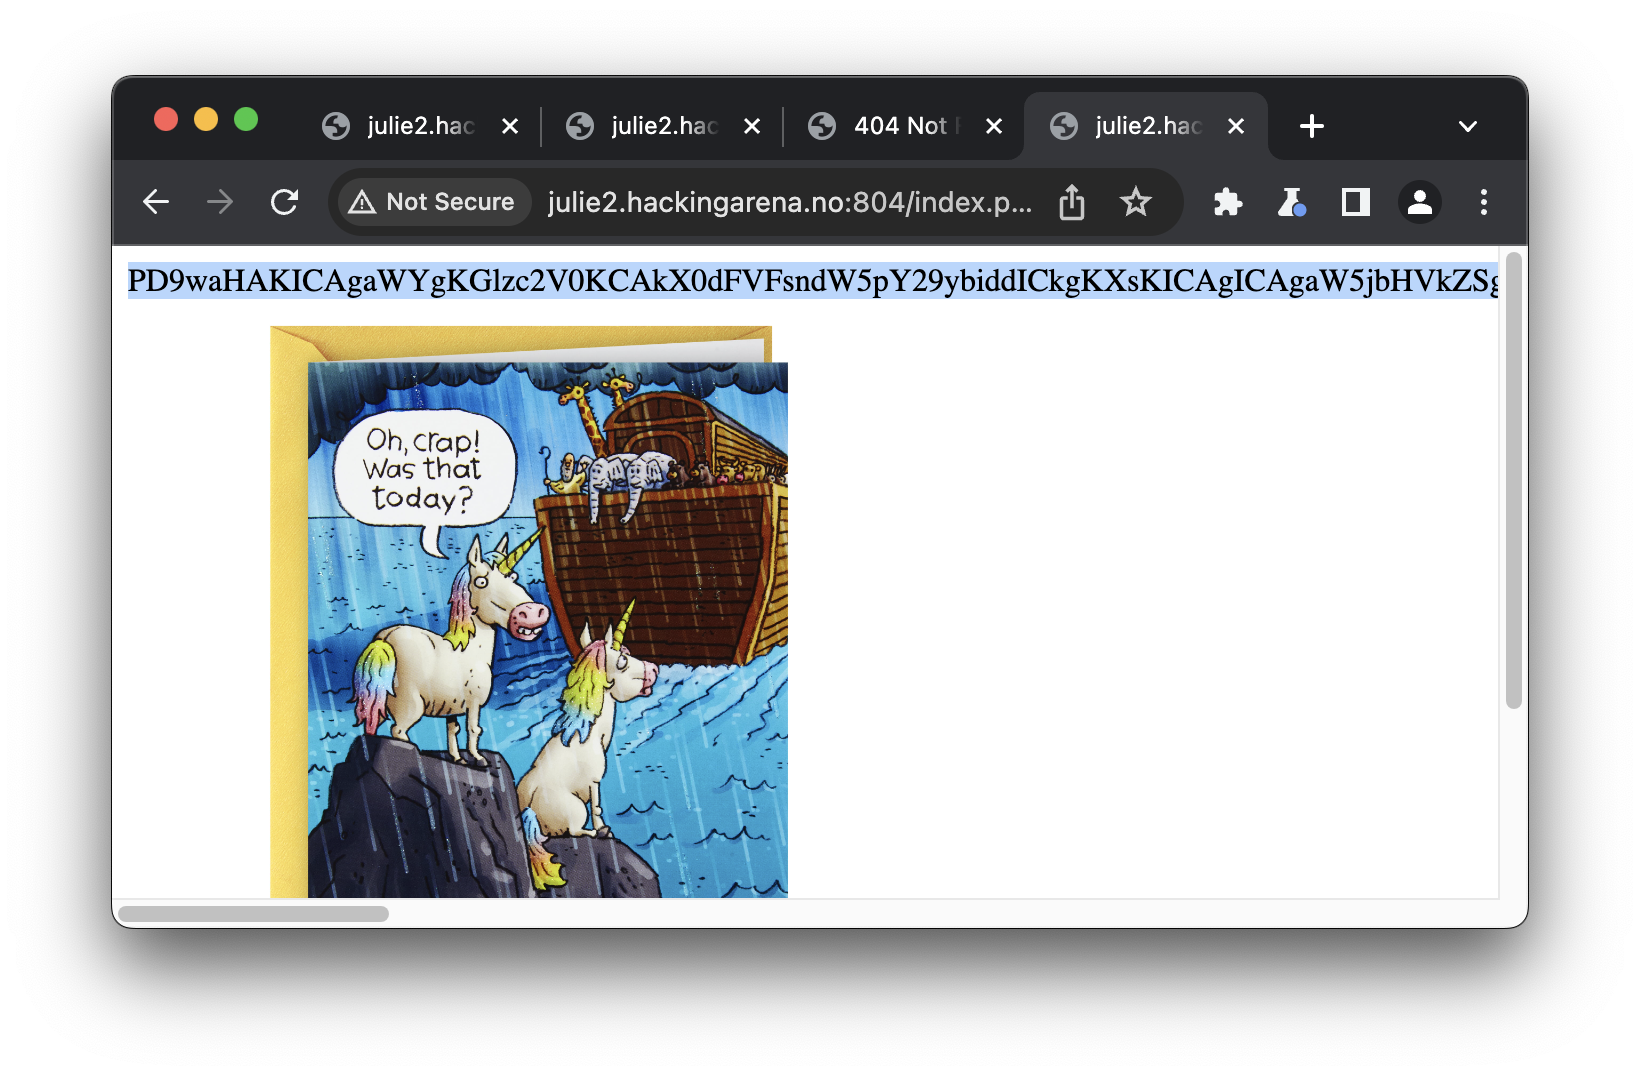
\includegraphics[width=12cm]{img/Web hacking/Order a Unicorn/Screenshot 2023-11-24 at 12.54.35.png}
\end{center}

Then I decoded it and found the following code:

\begin{center}
    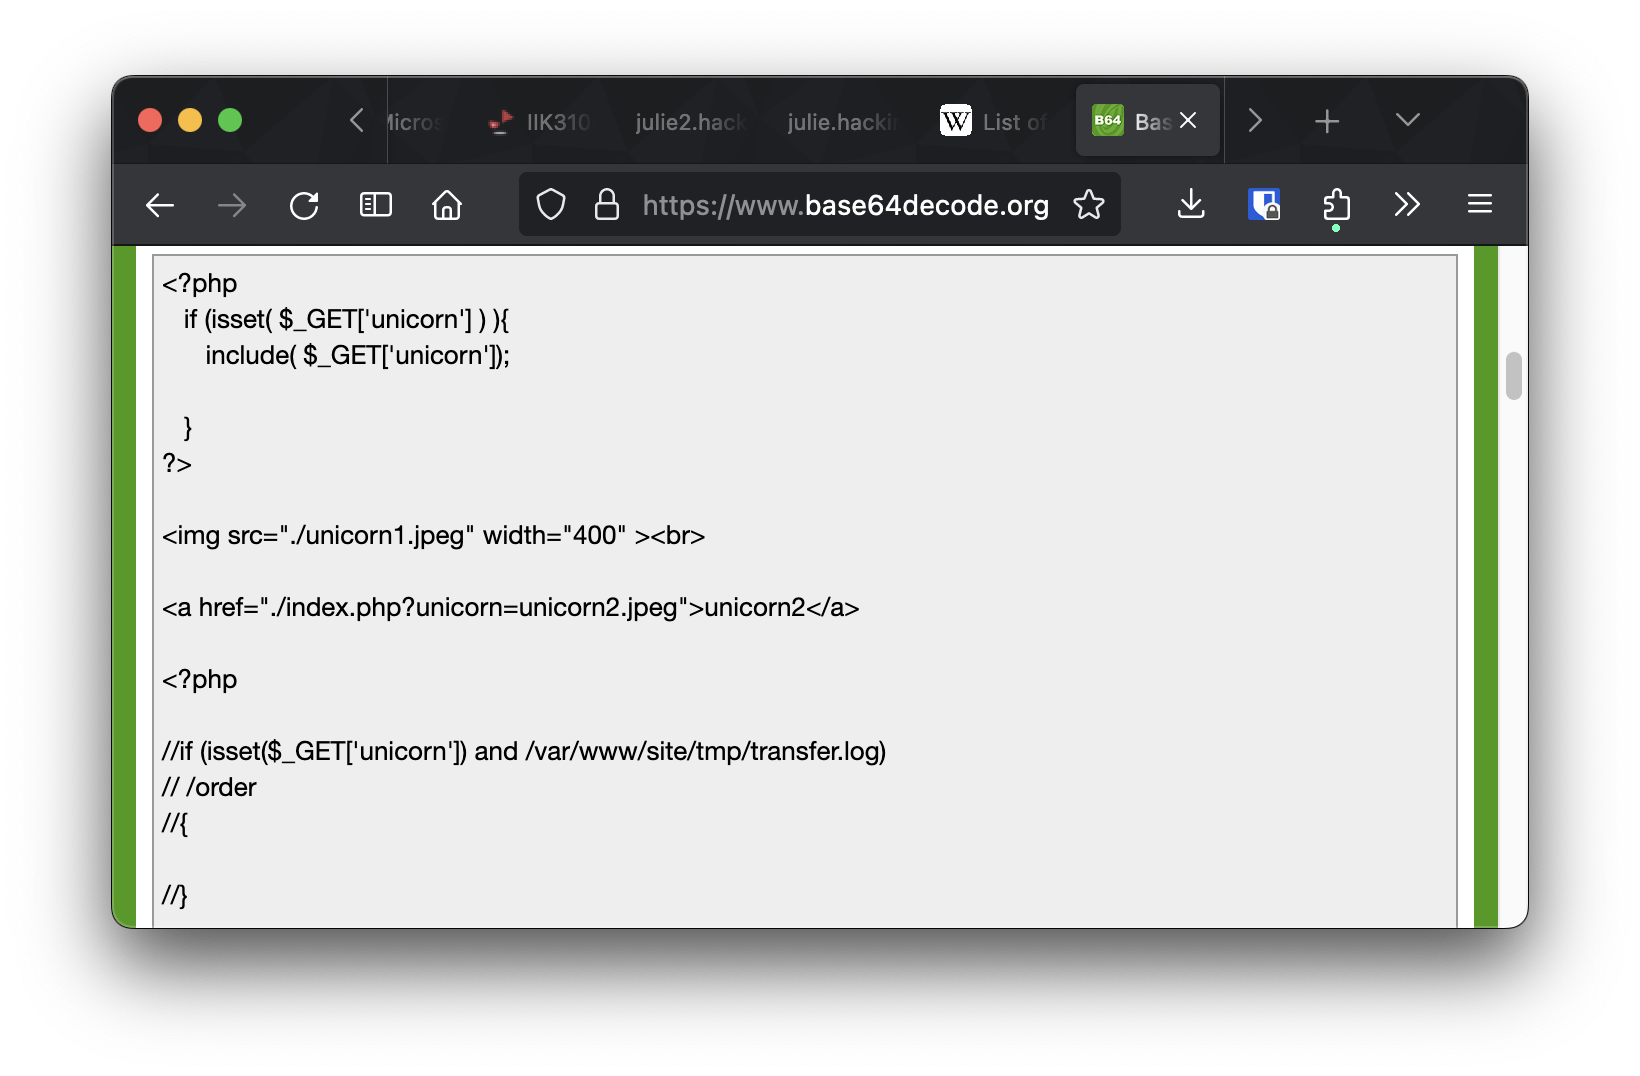
\includegraphics[width=12cm]{img/Web hacking/Order a Unicorn/Screenshot 2023-11-24 at 12.54.54.png}
\end{center}

I then looked at the \texttt{/var/www/site/tmp/transfer.log} that was revealed by the source code and found the following stride payment records:

\begin{center}
    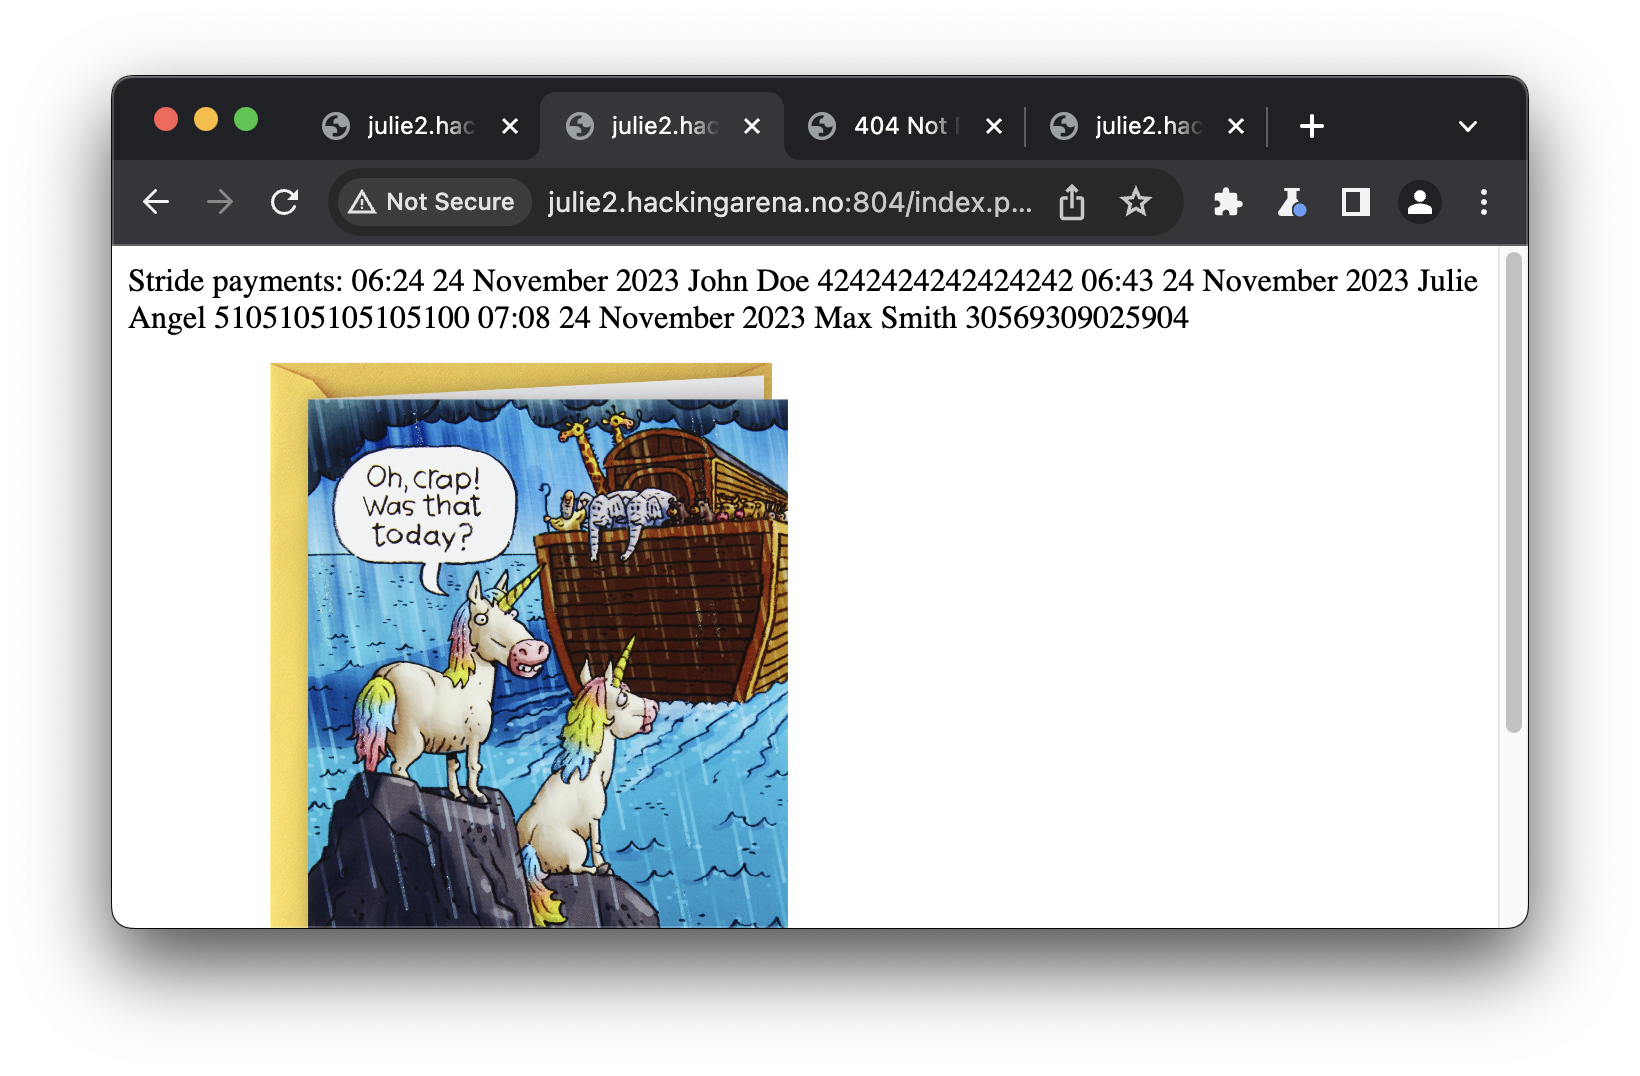
\includegraphics[width=14cm]{img/Web hacking/Order a Unicorn/Screenshot 2023-11-24 at 12.55.13.png}
\end{center}

I then when to the \texttt{/order} page and tried to order a unicorn with the card numbers from the stride payment records. But since none of them worked I started looking for example card numbers online and found a list from paypal test credit cards.

\begin{center}
    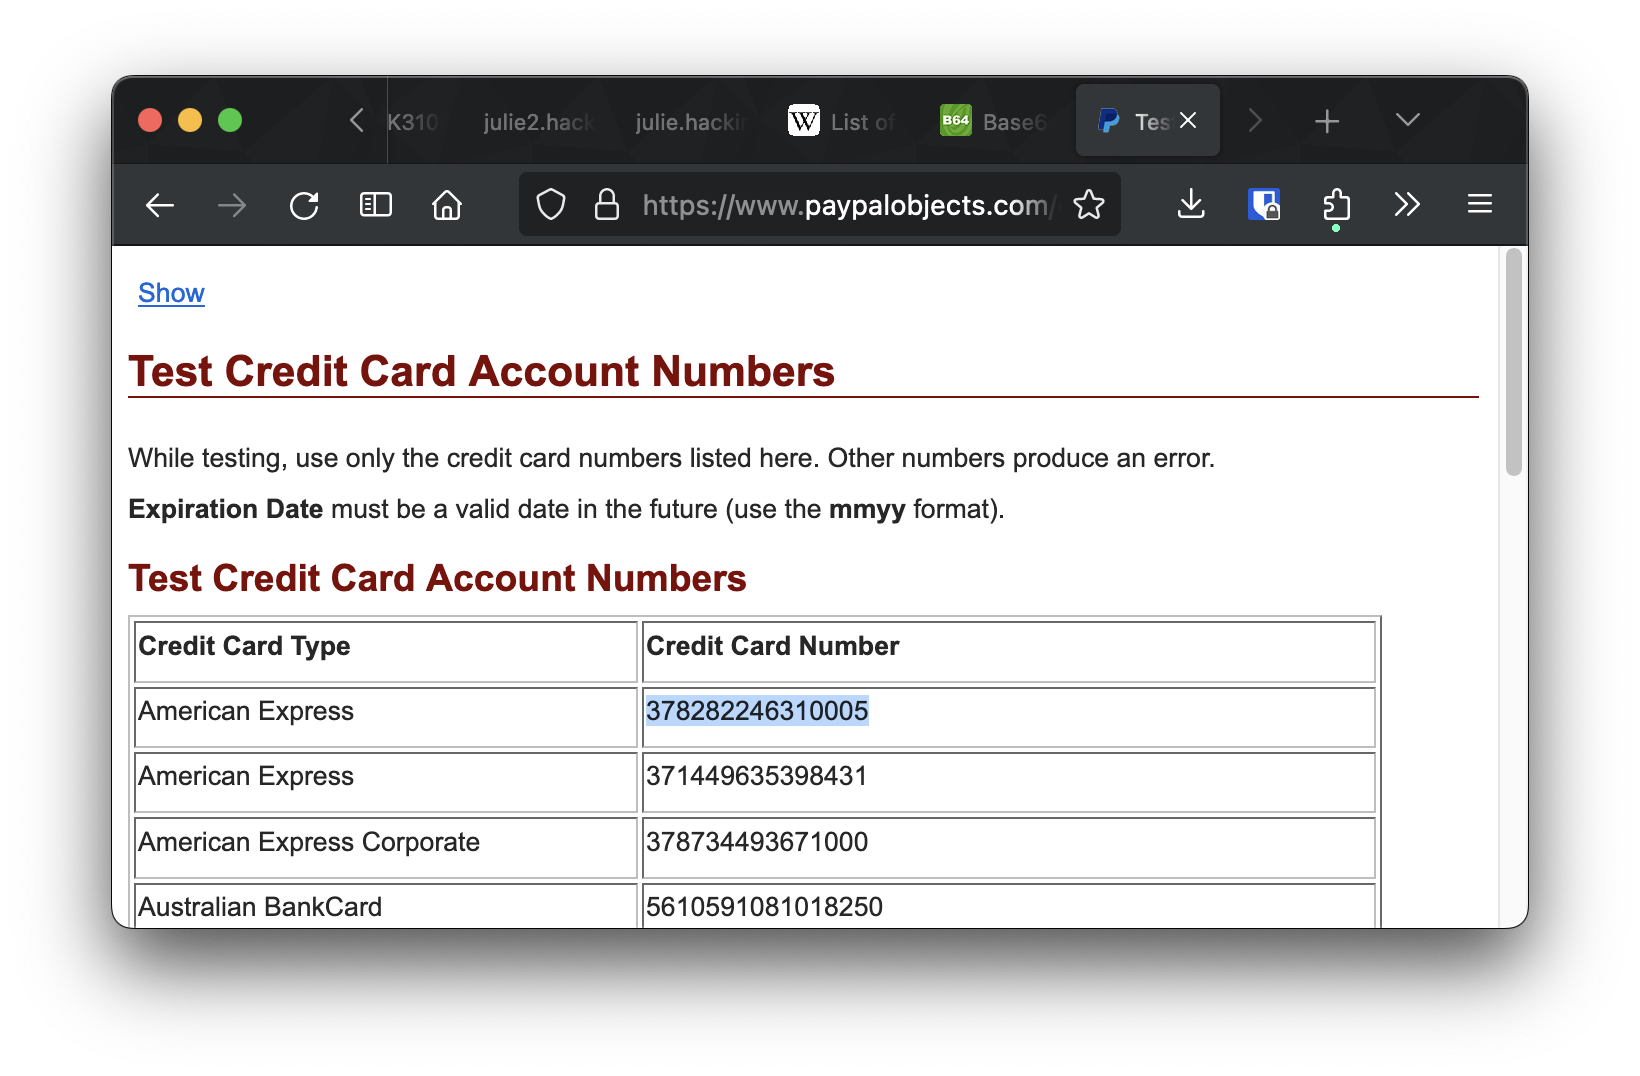
\includegraphics[width=15cm]{img/Web hacking/Order a Unicorn/Screenshot 2023-11-24 at 12.55.43.png}
\end{center}

I then tried to order a unicorn with the card number \texttt{378282246310005}...

\begin{center}
    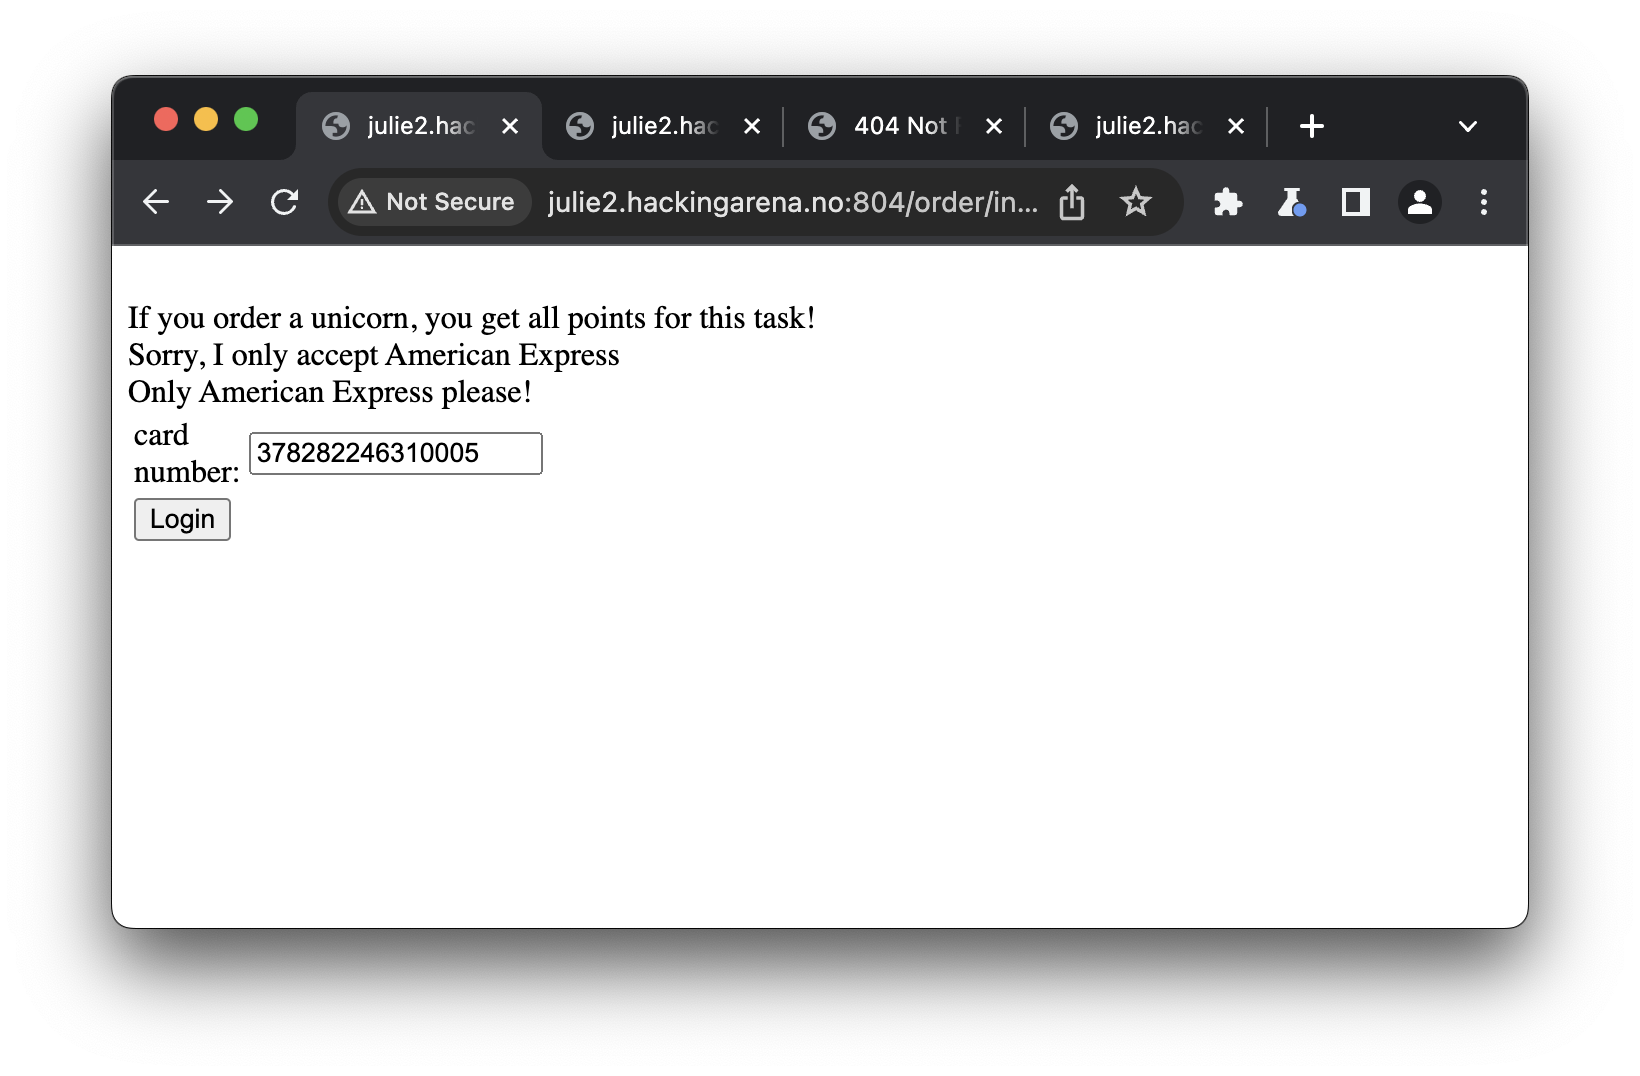
\includegraphics[width=15cm]{img/Web hacking/Order a Unicorn/Screenshot 2023-11-24 at 12.55.22.png}
\end{center}

...and got the flag.

\begin{center}
    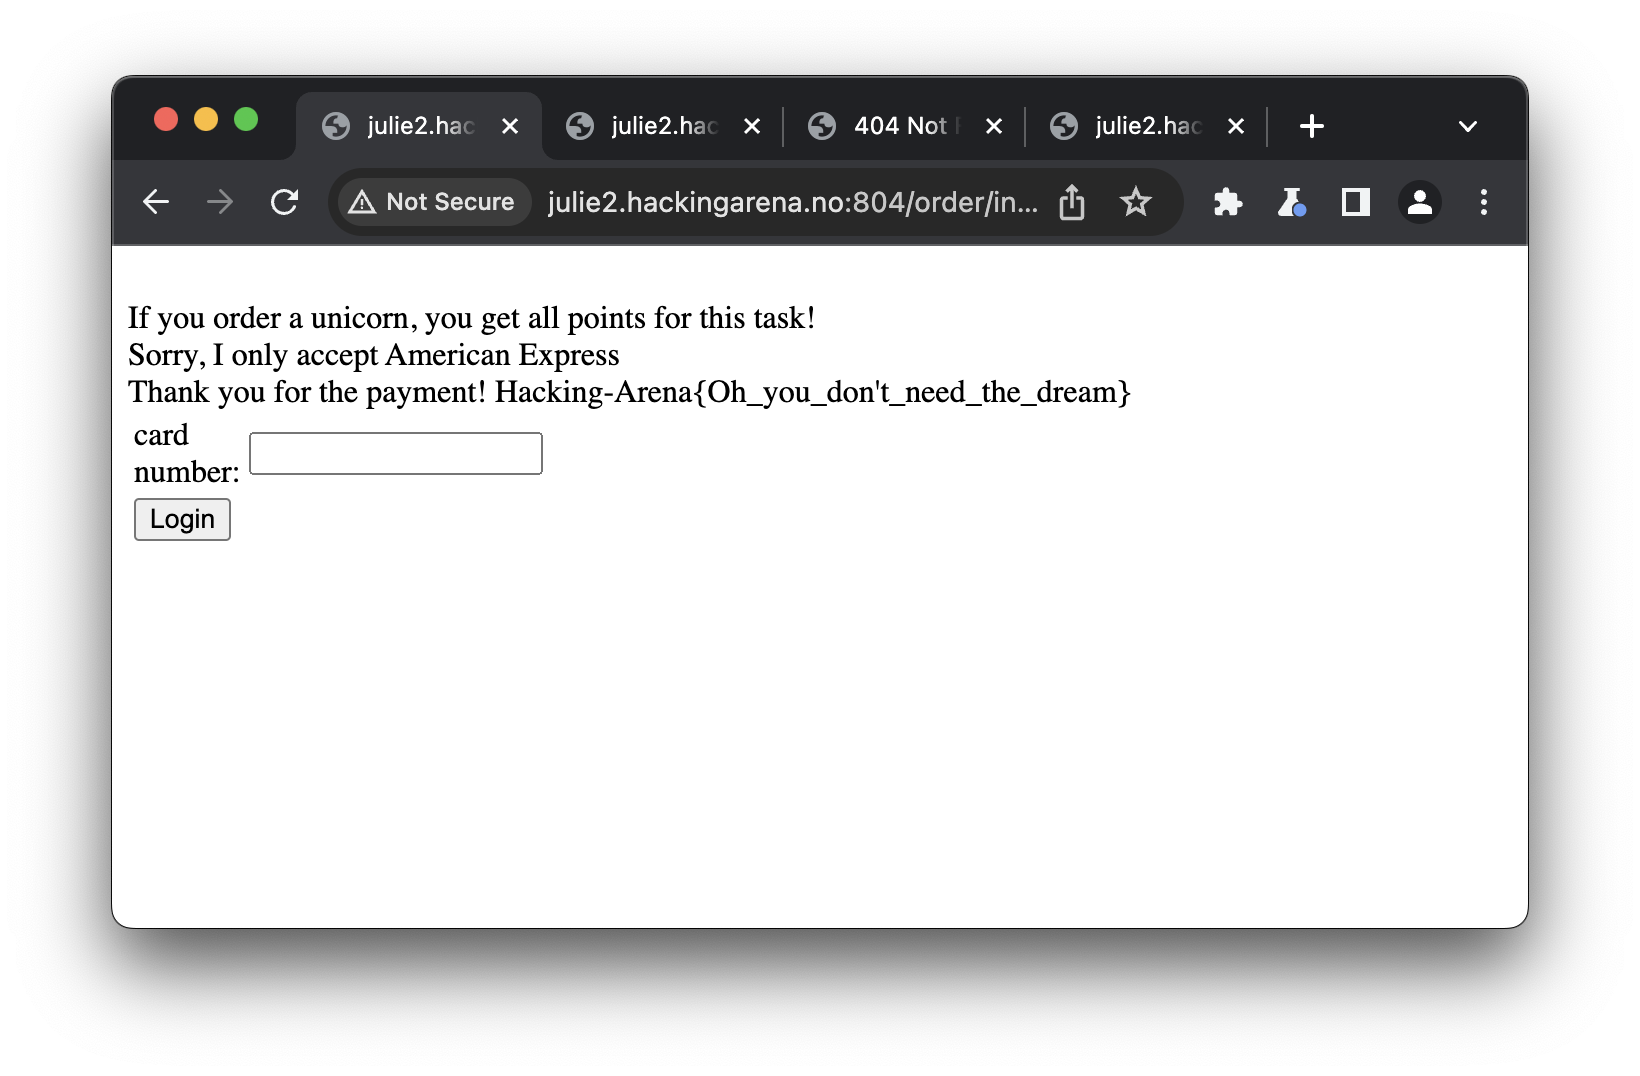
\includegraphics[width=15cm]{img/Web hacking/Order a Unicorn/Screenshot 2023-11-24 at 12.55.26.png}
\end{center}